\section{Timeline}

The following section describes the project development, progress and decisions we took through the time the project was developed. After a series of informal meetings, the project officially started in February 2012 and was submitted in September 2012.

\subsection{Initial Project Meetings and Early Implementation Decisions}

The regular project meetings where we discussed mostly the organizational aspects and the top-level design of the application started in December 2011. We easily agreed that we were aiming to create an application quite similar to Google Documents. We have decided very early to use a multi-tier architecture consisting of

\begin{itemize}
\item core translation memory,
\item user space,
\item graphical user interface,
\end{itemize}

\noindent which became very soon separate Maven modules, as we soon started using Maven for building the project.

After overcoming the problems connected with learning the new technology, we became quite satisfied with the decision to use Maven, because it enables to easily combine the parts of the project.

\subsubsection{Project structure}

Despite the fact that we added further modules later, we consistently kept the initial project separation into \emph{Core}, \emph{User Space} and \emph{GUI}. At the beginning, we also assigned team members to different parts of project, which remained relatively stable as well.

\subsubsection{Initial data}

Before receiving the data from OpenSubtitles.org, we were thinking about the source of data to fill the translation memory for the first time. There were several options -- either using the subtitle part of the Czech-English parallel corpus CzEng developed at ÚFAL \footnote{\url{http://ufal.mff.cuni.cz/czeng/}}, using sentences from a general purpose parallel corpus or getting the data from a subtitles server.

\subsubsection{Programming languages}

From the very beginning, we intended to base the project on Java, mainly because there are a number of web technology projects based on Java and
 every team member was familiar with the language. 
We also decided to combine the code in Java and Scala programming 
languages. At that time, there was 
only one team member who knew the Scala language. Although we 
repetitively expressed believes that everyone of us would learn it, at 
the end there was only one other person familiar with the Scala language.

The decision to use both Java and Scala appeared to bring a number of 
complications. On one hand, Scala allows to write concise and efficient 
code; on the other hand, most project members were not able to learn 
Scala sufficiently even to understand the Scala code properly, let alone 
actively producing Scala code, and only used Java.
Although the interoperability between Scala and Java works well in most 
cases because both are based on the JVM, some problems remain. One of the 
problems of interoperability was, for example, that a \emph{List} object 
created in Scala is not compatible with Google Web Toolkit, which expects 
a standard Java \emph{List} implementation.

\subsubsection{Technology for the Client: Google Web Toolkit}
\label{subsubsec:implementation:gwt}

Much more complicated to agree on was the technology of the client. There were many different opinions, from writing the client in {\it PHP} with {\it Nette Framework}, which some of us knew well, to using the {\it JSP} to have all the code consistently in Java, even to quite an extreme idea to make the whole application a {\it Java Applet} (this idea had appeared because of the intention to integrate the video player in the application, since at that time we did not know any other way to do that except creating a Java applet). Finally, we decided to use {\it Google Web Toolkit}, which no team member had any prior knowledge of, but it promised making the communication between server and client and many other things very easy. 

More information about the decision for using GWT and a discussion of its advantages and disadvantages can be found in Section~\ref{sec:reasonsForGWT}.

%Similarly to the Scala language problem, we ended up with only three people able to work efficiently with the Google Web Toolkit. Fortunately, this did not became a bottleneck of the development process.

% I guess me (Ruda) and Honza have probably mastered GWT, but Karel is also quite fluent in it



\subsection{Early Development Process}

Luckily for us, we very soon received a database from {\it opensubtitles.org} containing all the Czech and English subtitle files that were at the server at that time. Soon after that we started working on an alignment algorithm to retrieve the parallel data from the subtitle files (the process is described in Section~\ref{sec:aligning_subtitles}) and enable us to start experiments that helped us to decide which database system could be used.


\subsubsection{Database system}

Choosing an appropriate database system was also an intensively discussed issue. The database underlying the Translation Memory plays a crucial role for the whole system performance. Also using built-in features could save us a lot of additional work.
We evaluated different DBMS and decided to use \postgres~(see Section~\ref{sec:dbms} for details). To test its applicability for our project, we ran several small evaluations of \postgres~features that might be useful to us, e.g.\ the full-text search. As soon as we made the final decision on which DBMS to use, we refactored the evaluation code into {\tt TranslationPairSearcher} classes and started to set out the general architecture of the core. The {\tt BackoffTranslationMemory} class was added and the candidate search was finished in its early stages, so a basic version of the system could be used even though there were no sophisticated rankers yet. For more details on the core architecture, please see Section~\ref{sec:corearchitecture}.

Not having any experience with the object-relation mapping libraries in Java, we decided to use {\it Hibernate}, based on advice from both Internet forums and some of our colleagues.


\subsubsection{Data alignment}

Originally, all the algorithms processing the data we retrieved were implemented in Perl, and the code for importing the data was in the \emph{Core} module, implemented in Scala. Later, to make the code more consistent, we decided to move the data preparation and data import to a separate \emph{dataimport} module and to re-implement the Perl scripts in Scala.

\begin{figure}[h]
\begin{center}
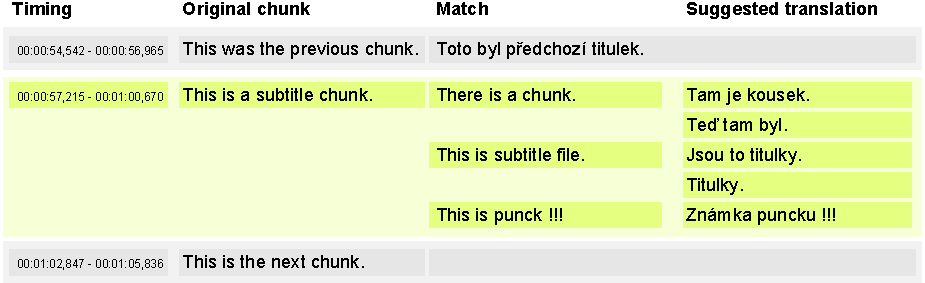
\includegraphics{./figures/original_strucutre.pdf}
\end{center}

\caption{Scheme of the originally intended structure of work with the translation memory. It reflects the original User Space structure and also schematically the original client design.}\label{fig:original_scheme}

\end{figure}

\subsubsection{Video playback}

Very soon, we started to try to solve the video playback in the browser, which we expected to be a really challenging issue. We did some research about \emph{Adobe Flash} technology. We were also thinking about creating a hybrid solution -- an application wrapper with a web browser inside, capable to ensure the video playback for the inner web application.

We very soon had toy implementations of:

\begin{itemize}
\item a player using VLC plugin, to be incorporated into the web application
\item a player as a desktop application, showing the web application in a frame (see Figure~\ref{fig:figures_desktop-app-player})
\end{itemize}

\begin{figure}[h!]
	\centering
		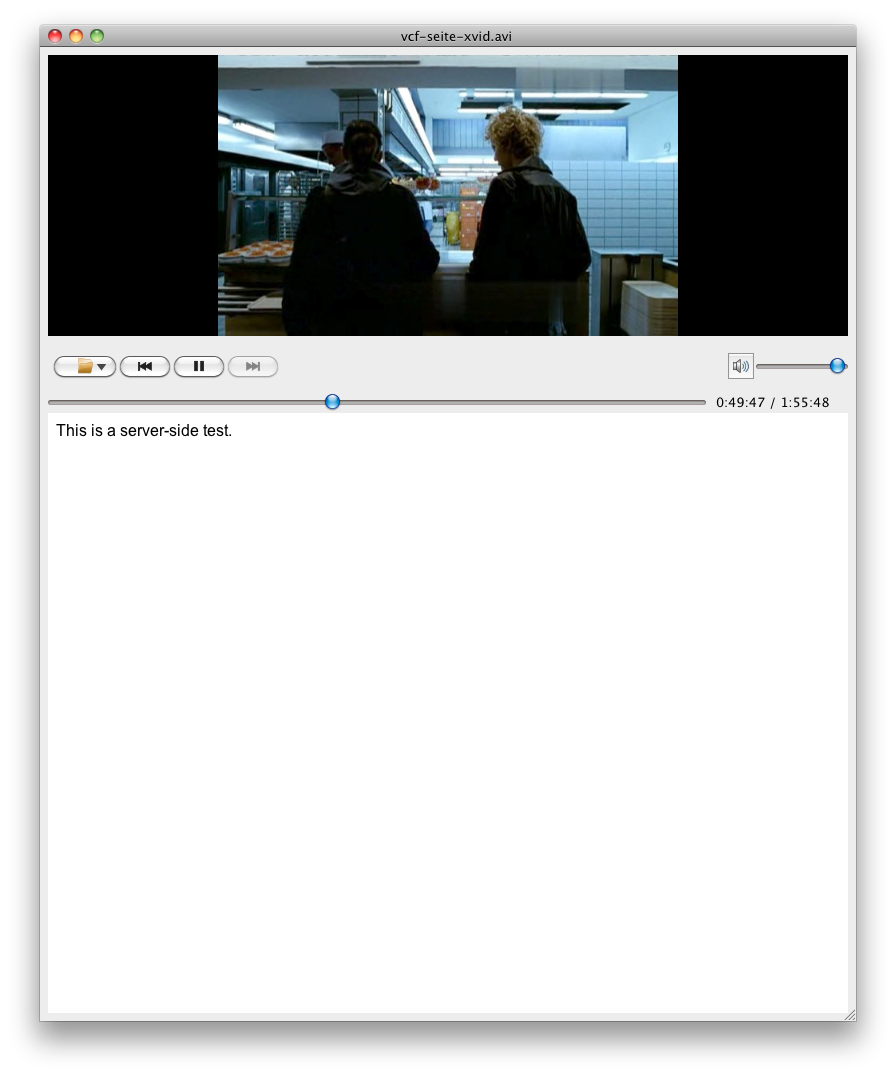
\includegraphics[width=7cm]{figures/desktop-app-player.png}
	\caption{Screenshot of Qt-based desktop application.}
	\label{fig:figures_desktop-app-player}
\end{figure}

We decided for the web application-only version, with no desktop variant, because, observing the development trends, it seems to us that the present and future of applications is in web applications. The benefits are e.g.\ that the learning curve is typically better for a web application, where the user is already familiar with most of the controls and work patterns, installation is not required, so anyone can start using the application immediately, it is easy to use OpenID registration.

Still, there are disadvantages, especially the cross browser support issues, limited power, and larger bandwidth consumption.
An added advantage of GWT is that the bandwidth consumption is actually closer to that of a standalone desktop app, because the application itself is stored in one JavaScript file, which is downloaded at the beginning (similar to installing a desktop application, but it is done transparently), and the rest of the client-server interaction is done through RPCs (basically the same way as it would be done in a desktop application).

An issue we encountered in developing the player and were not able to combat completely is letting the user choose a media file and passing its full file system path to the player. We found out that although it is quite easy to load a whole file from disc into memory, only its filename is passed to JavaScript instead of the full path for security reasons. We did a thorough search on the Internet but found out that there is most probably no clean way around this restriction.

Ultimately we came up with 3 solutions, but none of them pleased us enough:

\begin{itemize}
\item the user inputs the full path as a string into an input box; works well but is not user-friendly (most users probably do not even know that such a thing as a file path exists)

\item the user chooses the file in the file browser and then copies the file path from the browser input box into a textbox; this is probably even less user-friendly

\item a Java applet is loaded to choose the file as Java applets do not have such restrictions as JavaScript, and then passes the path to the application; it seems to us too heavy-weight to create and load a whole applet only to get the file path, but it works quite well -- except for the users who do not have Java installed and working properly (we have also encountered an alternative using Flash for the same purpose, but we still prefer using Java to Flash)
\end{itemize}

Despite having its disadvantages -- it is not particularly fast and from the users' view it could be considered not be really safe -- we decided for the third option.

\subsection{Introducing the Shared Classes}
\label{subsec:introducing_shared_classes}

After having implemented a very basic version of all three parts of the project, we decided it was time to start to solve the interoperability of individual parts in order to run a first snapshot of the application. This was happening approximately in March 2012.

At this stage we found out that we are not fully taking advantage of using the Java technologies for all parts of project and decided to totally redesign the User Space and Client parts.

Originally, we wanted to keep the traditional translation memory structure where each sentence can have several matches and these matches can have several translations in the memory, as is depicted in Figure~\ref{fig:original_scheme}. However, this scheme did not reflect much the way we worked with the data
in the Core, moreover there were not much cases where there would more translations for one match.

Also, the design of the GUI was a little bit confusing because the text of the matches was placed more prominently than the translation suggestions, despite the fact that the user is probably much more interested in the actual translation suggestions than in the matches. This lead to a modified scheme which is depicted in figure \ref{fig:new_scheme}.

\begin{figure}
\begin{center}
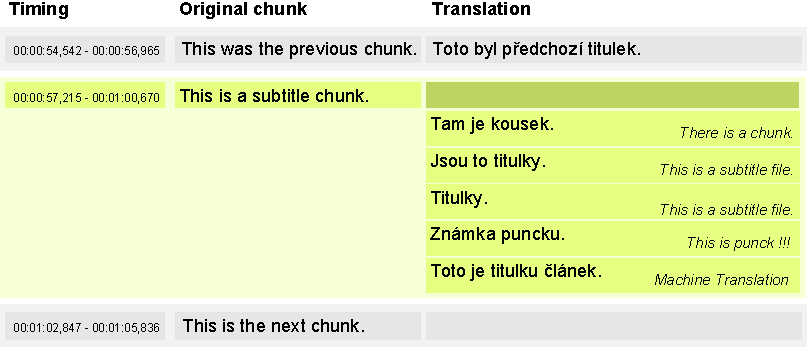
\includegraphics{./figures/current_strucutre.pdf}
\end{center}
\caption{Current scheme of the work with translation memory.}\label{fig:new_scheme}
\end{figure}

We agreed on the shared classes that all parts of the project should use. We more or less adopted the design of the classes from the core and started to use them in the whole project. This step required to re-implement some Scala classes in Java and to drop code that was already done in the User Space and the client. The design of the classes was almost the same as the final shared class design.

From a later point of view, it appears to be an important decision to agree on the shared classes, which made the cooperation between the modules easier and less verbose.


\subsubsection{GUI layout}

We started the work on the project with the new design soon, which lead to a period of struggles with technologies. It took us almost two months to have the first running version of the application.

The very first version of the application was a page where it was only possible to upload a subtitle file and to do the translation, without any possibility to load an already saved subtitle document or download the result of the translation, without any sessions or users; it was just a page where you edit the subtitles (which later became the Translation Workspace).


\subsubsection{External APIs}

At that time we used machine translation from the MyMemory service (which in fact wraps Google Translate), but there is a limited access per IP address and we soon began to reach the limit very frequently. It became obvious the we would have to change the source of machine translation. Based on that we decided to train our own Moses system. See Chapter~\ref{chap:moses} for details.

We also used an API providing IMDB.com information to receive information 
about movies but the movie meta data was not used in the evaluation the 
matches at that time. We had to switch to Freebase later because the IMDB service we used was discontinued.

\subsection{The Main Development Phase}

It is hard to define the main development phase which is covered in the 
following paragraphs. It corresponds to the period from the beginning of 
March when the important design changes were made (see previous 
Section~\ref{subsec:introducing_shared_classes}) to approximately the 
middle of August when adding new features was stopped (see the next 
Section~\ref{subsec:final_development}).

The section is divided to parts covering the issues we were dealing with 
and describes what we did in each area in those approximately five and 
half months.

\subsubsection{OpenID}
\label{subsubsec:openid}

Although we wanted to implement OpenID support from the very beginning, 
we started with it approximately in May. We found the two most frequently 
used Java libraries for OpenID and tried them. Those were \emph{JOpenID} 
and \emph{openid4java}.

\emph{JOpenID} seemed to be easier to use and also was much smaller as a 
dependency; on the other hand, when we ran into some problems with using 
it, we found out that \emph{openid4java} is much more frequently 
discussed on the \emph{StackOverflow.com} forum and that there is a 
bigger chance that we would be able to find some advice for potential 
problems. 

However, as discussed in \ref{us:openid}, \emph{openid4java} is easier to implement, so we used that, even for its biggest shortcoming -- users are not able to set their own OpenID provider.

The support for OpenID was finished in July, the parser for the authentication data from Seznam was added at the beginning of August.

\subsubsection{Chunk Splitting}

An interesting issue, also from the linguistic view, we had to solve was to find the best way of splitting the subtitle items into chunks. As opposed to the classical way of simply splitting documents into sentences, we had several possible ways of doing the splitting because of the nature of subtitle files.

We talk about chunk splitting more in chapter~\ref{os:sentence_splitting}.

We then realized that it is important that the splitting the same when importing subtitles into the database and when processing the user subtitles (as discussed in~\ref{os:guiparsing}), so we made it a shared class.

%\subsubsection{Chunk Time Format}
%
%% Originally, we simply used the time strings acquired from the subtitle files to represent the timing, as we only displayed them to the user.
%% 
%% This was sufficient at the beginning; however, once we began fitting the media player to the actual subtitle lines, we needed to parse the time strings and convert them to a one-ineteger representation of time in miliseconds (we also needed that for editing the timing, which came later).
%
%After a period of representing the time simply as a string, we created a class, {\tt SrtTime}, that represents the time in the SRT format as a set of four integers (the SRT format of time is ``hh:mm:ss,ttt'' -- hours:minutes:seconds,miliseconds).
%%\footnote{a milisecond is a thousandth of a second, thus the usage of the letter ``t'' to represent it; alternatively, knowing that the word ``second'' stands for the second diminuation of the hour, you can think of the milisecond as a third diminuation of the hour, also leading to the letter ``t''}).
%We then decided to move all time handling logic into this class, so that we can ensure the correctness and consistency of the timing throughout the application.
%The class provides various constructors, getters and setters for all formats we need, also performing validity checks.
%% (one string, a set of strings, a set of integers, one integer being the time in miliseconds). It also implements cloning, comparison and subtraction.
%
%At first, we decided to use the SRT format only for the sake of simplicity.
%It was thought to be only a temporary state, with a plan to add SUB format support later. However, we eventually found out that not only is the SRT time format easier to use (it is not necessary to know the Frames-Per-Second property of the movie file),
%but as we saw in the opensubtitles.org data (see section~\ref{sec:properties}) also approximately 99\% of subtitles on the Internet appear to be in the SRT format.
%Thus, we decided to discontinue support for the SUB format and only support SRT (the only major difference between these formats is actually the format of the time).

\subsubsection{Chunk Annotations}

The initial reason for annotations on the chunks was for the Named Entity Searcher, which marks Named Entities such as Person, Place, Organization in the text and the user should be able to correct those if they differ and source and translation.

Later, another level of annotation was that chunks are often split by dashes denoting individual dialogue speakers. The dashes need to be removed for generating suggestions because they are irrelevant for this step, however they need be kept for correct rendering of the text.

Other annotations include newlines, which are often part of the chunks to ensure that they fit on a single screen. Again, the newline character is irrelevant for generating translation suggestions, but it is necessary to render the subtitles properly.

Another possible annotation is subtitle formatting for bold, italic and underlined text. Initially, we wanted to extended the annotations again. However, it seemed to be too complex, especially in the GUI, so we decided to strip off subtitle formatting in the current version of the application. The reason for this is that it is used very little and there is no formal specification, which means that there exist various formats. Often, media players do not support the formatting properly, so we want to discourage the users from using the formatting.

A Chunk has a set of methods to retrieve and set the annotations correctly, using the notion of forms. The forms used are:

\begin{itemize}
	\item \emph{database form:} the text as stored in the subtitle file, only cleaned -- formatting stripped off (bold, italic etc.), non-printable characters turned into spaces, multiple spaces replaced by one space only and newlines are stored as PIPE characters.
	\item \emph{surface form and annotations:} the surface form is the text to be used to generate the translation suggestions, without dashes and with newline turned into spaces
	\item \emph{GUI form:} the HTML form to be displayed in the GUI. Newlines are turned into {\tt <br />} tags.
	\item \emph{text form:} the form to be used in HTML textareas -- with dashes, newlines are generated as {\tt \verb#\n#} characters.
\end{itemize}


\subsubsection{Logging}

In User Space and Core, we use Log4J, which implements the standard Java Logging interface for logging.

The situation with the GUI is not so easy. GWT provides some default logging tools which are able in while running the application in the development mode in IDE, anyway it does not provide tool for logging a common run of the application.

Originally, we created a debugging console which was present directly in the user interface which was only a temporary solution, because it is 
certainly not a good practice to show such technical details to an end user.

The final solution we took is what we call ``remote logging''. Important messages are now sent to the server through an RPC, where they are both included into the server log and saved into the database for possible future use (together with the {\tt userID} if possible).
The minimal level of a message to be sent to the server can be set (debug, info, warn, error). We log important GUI events and mainly exceptions with their stack traces in order be able to react on potential bug reports later.

There appeared some technical difficulties -- catching unexpected exceptions in GWT and umbrella exceptions. an umbrella exception is an exception thrown when multiple exceptions have occurred at once, and contains all of them. Its message and stack trace are not useful at all because they only cover the creation and throwing of the umbrella exception itself, but do not reveal anything about the inner exceptions.

This was solved and the remote logging mechanism was ready to use at the beginning of August.

\subsubsection{Implementing the RPCs}

From the start, it was obvious to us that we want to use a well-established method to implement the Remote Procedure Calls.
We noted in the specification that we would probably use JSON for the message serialization.
Fortunately, GWT does provide a ready-to-use Remote Service implementation, where the programmer only has to define the set of RPCs as an interface, implement the interface on the server side, and invoke an RPC on the client side by implementing the GWT {\tt AsyncCallback} interface.
Everything else is handled automatically by GWT (which, as a matter of fact, does actually serialize the messages to JSON internally).

The type of an RPC parameter or its return value can be any GWT-compilable type. Because this type must be known both to the server and to the client, we use only primitive types and shared classes. Each class sendable through the GWT RPC mechanism must implement the GWT {\tt IsSerializable} interface (which is only a marker, i.e.\ it does not have any abstract methods) and a parameter-less constructor; this also holds for the checked exceptions, which are technically only a special type of a return value.

Because of JavaScript and browser limitations, the RPC mechanism of GWT only allows asynchronous calls from client to server. This suited our needs often, but we had to go around these limits in some situations. Quite often, we need the RPC to be synchronous and blocking, e.g.\ in logging in or changing user settings. In such situations, the page or dialog is ``deactivated'' on invoking the RPC (all active components are disabled -- e.g.\ the text boxes are read-only, the buttons do not respond to clicks), a reference to the page or dialog is passed to the class invoking the RPC, and when the RPC returns, the page or dialog is ``reactivated'', either with a success message or an error message, depending on the result of the RPC.

In one case, we would need an opposite direction RPC, i.e.\ the server to invoke the RPC on the client. This is when authenticating the user through OpenID, where we have to perform the authentication in a new window -- the new window then receives the result of the authentication, but it cannot be easily passed directly into the opener window. Here, we decided to use active polling -- the opener window regularly invokes the {\tt GetSessionID} RPC, which returns null if the authentication process has{ not yet finished, this being a signal for the GUI to continue polling. To link together the opener window and the authentication window, a unique {\tt authID}, generated by the User Space, is used.

\subsubsection{Failed RPC Requests Handling}

We decided that our general error handling strategy should be to try to solve all problems without user interaction, and to inform the user only about user-generated errors (such as incorrect SRT file format or session timeout) or critical errors (such as permanent loss of connection to server).

The first thing was to turn the calls into objects, so that they store their parameters and can be called again on failure. We also created a generic superclass for them, Callable, filled with the necessary boilerplate code and methods performing the default actions, to be overridden if necessary.

We identified the response that we usually get in case of network problems (it is a {\tt StatusCodeException} with the status code 0). The problems can be temporary or permanent; in case of temporary problems, the default response of showing an error message was found to be highly inappropriate, as it would suffice only to resend the call. Therefore, we introduced retrying the call for three more times in such case with short delays, before showing an error message to the user.

The retrial of calls has proven to be an efficient way to deal with problems, so we decided to extend it to all types of failures. However, in case of non-network errors, we soon found that retrying the calls does not make sense in some situations; so we decided to keep the retrial as a default action which can be overridden in the extending classes.

We also added a timeout for each request after which the request is regarded as lost and is retried. Such a situation is not at all typical, but we need to expect  it to prevent the user from ``starvation'' (the user can always escape from any state by refreshing the page in the browser, but this can lead to an uncontrolled local data loss or even to objects being left in an inconsistent state -- such as a document without content).

\subsubsection{Sending Translation Results}

At first, the translation suggestions from the Translation Memory were requested and sent for each chunk individually. This had the theoretical advantage that the user received each of the translation suggestions as soon as possible. However, we found the overhead of the RPC calls to be unreasonable. Not only was the overall time necessary to load all the suggestions too long, but also a typical browser was unable to handle such a large number of requests and usually froze for long periods of time, often unfreezing only after all of the suggestions arrived.

A simple solution seemed to be sending all of the chunks for translation in one request. However, such a request can take several minutes to complete, and we still wanted to keep the nice property of the application of showing the suggestions as soon as possible at least for the first lines -- so that the user can start the translation immediately. Thus, we decided to send the request in batches, starting with a small size of the batch for the beginning of the file and gradually increasing the batch size.

The first way to do that was an exponential increase, where each batch contains twice as many chunks as the previous one, starting with a batch of size one. This proved to solve the aforementioned problem of browser freezing; however, another problem arose. As the batch sizes grew larger and larger, the later requests often took several tens of seconds or even minutes to complete. Meanwhile, the user would often navigate away from the Translation Workspace, rendering the translation suggestions, including the currently being processed ones, obsolete. This was of course detected in GUI and the suggestions were thrown away on arrival, but still it meant that the server was working in vain for some time, possibly resulting in an unnecessarily slower responsiveness to other users (and even to the very same user as well).

We introduced two further solutions. The first and simple one was limiting the size of the batch to 64 chunks (which typically take at most 5 seconds on the server side), so that the amount of useless work could not grow too large. The second solution was to stop the translation suggestions from being generated on the server, by issuing a {\tt StopTranslationResults} request. (This breaks the typical model of processing the queries, where once a query is sent, its processing is not influenced by queries that arrive later.)

The two major issues with the {\tt StopTranslationResults} request were:

\begin{itemize}
	\item to interrupt the suggestions generating which is already in process (which is done in parallel for the chunks in the batch, making this even harder).
	\item to identify what to stop and what to let continue.
\end{itemize}

The first idea was to mark the whole document as closed, and to check this when generating the suggestions. However, this would cause problems if the same document was immediately reopened by the user, and even larger problems if the user already had the document opened twice -- this can easily happen by mistake, the logical reaction of the user is then to close one of the Translation Workspaces, and then he would stop receiving suggestions even in the other opened Workspace. Thus, we then decided to create an identifier for each Translation Workspace instance and to bind the {\tt StopTranslationResults} request to this identifier. However, we soon found out that this would require additional overhead only to handle this probably not very common situation, so we dropped that idea as well.

Finally, we decided for a compromise solution between those two. The {\tt StopTranslationResults} request is now bound to individual chunks, which now have an added boolean field {\tt isActive}. This field is set to true when the {\tt GetTranslationResults} request arrives to the server, for each of the chunks on the request. The {\tt StopTranslationResults} request contains a list of the chunks which translations should be stopped. On arrival of that request, the User Space simply sets the {\tt isActive} field to false -- because User Space and Core share the same memory and because only references to the chunks are passed around, this change is visible in core even though the chunks have already been sent for translation. The necessary overhead is minimal, and there is no "false alarm" in the typical case. The only unsolved case is the situation where the same batch of chunks are sent for translation at the same time from two different instances of Translation Workspace with the same document opened, and then one of these Workspaces is closed, causing the suggestion generation to stop even for the batch from the other Workspace. Although this situation is unlikely and non-critical (the suggestions would be missing only for this one batch, the later batches would be translated correctly), we still offer a general solution by repeating all request on failure (unless it is obvious that the failure will reoccur).

Finally, we decided for a compromise solution between those two. The {\tt StopTranslationResults} request is now bound to individual chunks, which now have an added boolean field {\tt isActive}. This field is set to true when the {\tt GetTranslationResults} request arrives to the server, for each of the chunks on the request. The {\tt StopTranslationResults} request contains a list of the chunks which translations should be stopped. On arrival of that request, User Space simply sets the {\tt isActive} field to false -- because User Space and Core share the same memory and because only references to the chunks are passed around, this change is visible in core even though the chunks have already been sent for translation. The necessary overhead is minimal, and there is no "false alarm" in the typical case. The only unsolved case is the situation where the same batch of chunks are sent for translation at the same time from two different instances of Translation Workspace with the same document opened, and then one of these Workspaces is closed, causing the suggestions generation to stop even for the batch from the other Workspace. Although this situation is unlikely and non-critical (the suggestions would be missing only for this one batch, the later batches would be translated correctly), we still offer a general solution by repeating all request on failure (unless it is obvious that the failure will reoccur).

\subsubsection{User Management}

At the very beginning the GUI was basically only the translation workspace. It was possible to translate a subtitle file in the application, the changes were reflected in the database, however it was not possible to get them in the application when the web application was reloaded or to export the subtitles.

We considered the user management to be just a minor technical issue. However, to enable to reach the intended architecture of the User Space -- mostly that most of the calls should be resolved in the Session objects -- we introduced a simple fake login in April (you could log as any user using password "guest").

We started to implement the OpenID login support in May (see Section~\ref{subsubsec:openid}). When we met some technical difficulties, we decided to implement our own registration and login first.

Because our own experience was that requiring a registration from a web service often prevented us from using it, we decided to make the registration as easy as possible. We have no constraints on user names (except for non-emptiness) and very little constraints on password (only it must be at least 3 characters long).

We think the most important feature of a password is for the user to remember it, so we leave the assessment of the strength to the user. The password strength constraints are often rather arbitrary and many classes of strong passwords do not pass them, it is hard to develop a reasonable strength measure. E.g.\ a whole sentence, a "passphrase", is a very strong password; however, it usually does not pass measures requiring use of specific classes of characters. And vice versa, a password using very unusual characters (e.g.\ Czech letters with diacritic signs) can be impossible to break even if it is quite short, because the attacker simply does not try out such characters that are uncommon in passwords; still it often does not pass typical minimum password length constraints.

Moreover, we are not forced to pay much attention to the security of the application - it does not contain any sensitive data whose compromising would pose a threat to the users of the application and the benefit to the attacker successfully breaking into a user account is close to none.

We allow the user to work in multiple browser tabs or windows, provided it is the same session (i.e.\ it has the same {\tt SessionID}), because we believe it is natural to work on multiple translations at once, to have the Document List opened to see the translation progress, etc. The user himself is responsible for having the same document opened multiple times, which is not expected behavior and so changes to the document in one Translation Workspace are not projected into the other Workspace until reloaded.

However, we decided to disallow one user having multiple sessions at one time, as we believe that this is neither expected nor required behavior, and could potentially confuse the user. We believe that such a state is usually caused by a mistake, e.g.\ user A forgetting to log out on PC 1, then moving to PC 2, and at the same time user B using the application on PC 1 under user A's account by mistake.
We do not support multiple users collaborating on one subtitle file at the moment.

If a user registers through OpenID, we have to assign a user name to him (the unique OpenID identifier we get is typically a long hash, which does not look like a nice user name), see Section~\ref{subsubsec:gui_openid}. Because the user name is at least partly generated, the user might not like it. Therefore, we offer each user the possibility to change the user name (provided that the one he chooses is free). The user name is only used to authenticate the user (if not using OpenID login) and is displayed in the top right corner in the application; the internal unique identifier of a user is his user id, an integer assigned to each user on registration that never changes.

\subsubsection{GUI Look and Feel}

After using default GWT look, we decided to use Twitter Bootstrap, which turned out to be a good decision as it looks decent and provides additional widgets.

\begin{figure}
\begin{center}
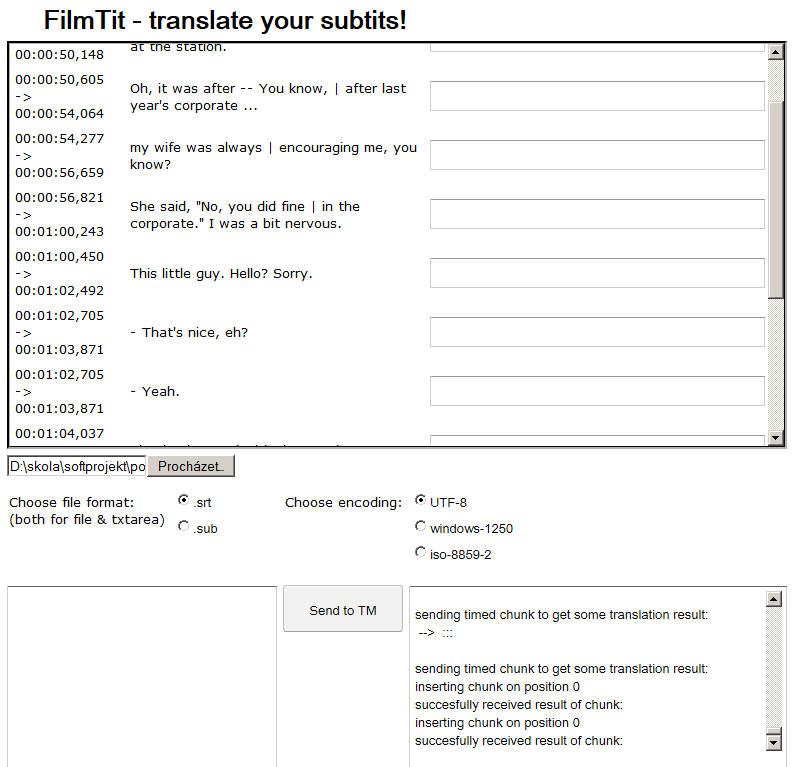
\includegraphics[scale=0.5]{figures/old_screenshot.png}
\end{center}
\caption{Design of the Translation Workspace before starting to use the Twitter Bootstrap}
\label{fig:before_bootstrap}
\end{figure}

Trying to be user friendly

\begin{itemize}
\item expected behavior
\item as litle controls as possible
%- can be controlled by mouse %(except for typing)
\item TranslationWorkspace can be controlled both by mouse and by keyboard, as the user is expected to spend most of the time in Translation Workspace by typing, and the need to switch between the mouse and the keyboard would decrease his efficiency
\item other pages controlled only by mouse, which feels natural enough; a typical user spends most of the time in Translation Workspace, therefore having to use the mouse on the other pages is not expected to be an efficiency problem
\end{itemize}

changing data .. idea: it should be possible to change anything if there is not a strong reason why not
\begin{itemize}
\item change document title, movie title... by clicking on it (seems natural, added a tooltip)

\item change timing or source text: we think that this is not usually required so it is under a double click to prevent unwanted activation (and a tooltip again)

\item we offer the user the possibility to change the source text because if there is an error, the suggestions might be incorrect (the suggestions are regenerated on changing the source)

\item we do not offer deleting chunks because this would be difficult to implement properly in GUI; however, the default behavior is not to export the untranslated chunks, so not translating a chunk is roughly equivalent to deleting it

\item we do not allow to change the source subtitle file (this would actually mean deleting the whole old document and creating a new one, probably only keeping the title -- so we leave this for the user to do himself); however, smaller edits can be done directly in TW
\end{itemize}

\subsubsection{GUI Pages}

We started having one page only, the Translation Workspace, which was sufficient for development of the application for several months. Later we added the Document  Creator page as the default one, which replaced itself by the Translation Workspace once a document was created, and this was sufficient for some more time. However, we eventually could not avoid adding more pages and the need to explicitly handle multiple pages became obvious.

We immediately found out a week point of GWT here: it has nearly no native support for multiple pages. This was quite a surprising issue to us, since in any other web development technology or framework that we know, creating a new page and switching pages are really simple tasks. GWT, however, observes the idea of having one HTML file and one JavaScript file only that handle everything. (It is technically possible to create multiple pages by creating multiple GWT projects, each corresponding to one page, but this is not recommended for many good reasons.)

The GWT way of switching pages is by replacing the contents of the Root Panel (which represents the visible part of a page), or any other Panel placed within the Root Panel (which we decided to use so that some elements, such as the menu, are present on all pages). The switching is done without reloading, simply by creating an instance of the new page and directly setting it as the contents of the panel (without any convenience functions for that to our knowledge).

All the pages have the same URL by default, but GWT offers the History class for changing the URL and reacting to changes to URL (however, it is not linked to page switching by design -- this remains for each programmer to do by himself). There are also {\tt Hyperlink} widgets, which represent a link to a different page, with the default action being changing the URL and invoking the appropriate handler (a {\tt ValueChangeHandler}).
The URL contains an anchor with the name of the page (e.g.\ {\tt \#DocumentCreator} or {\tt \#WelcomeScreen}), and the History class is able to provide the name of the anchor to the user and to invoke the ValueChangeHandler when the URL changes.

We decided to use the {\tt History} class and {\tt Hyperlinks} to implement the menu and page switching. We create a {\tt PageHandler} class which implements the {\tt ValueChangeHandler} -- it turns the anchor string into a value of Page enum, checks whether the requested page can be loaded (especially based on the user log in / log out state) and loads the appropriate page. It also provides public methods to other parts of GUI so that they can switch pages, modifying the URL at the same time (so that the browser refresh works as expected).

However, we encountered one issue with the {\tt Hyperlinks}: the {\tt ValueChangeHandler} is invoked only if the value of URL changes, which means that if the user clicks a menu link which points to the page loaded (e.g. while creating a document, the user decides to restart and clicks the document creator link), the handler is not invoked. As this behavior is hard-coded into the {\tt Hyperlink} class, we had to abandon the Hyperlinks and used {\tt NavLinks} instead (a simple link with no default interaction with the History), with click handlers invoking the {\tt ValueChangeHandler}.

%When reviewing the resulting code, we found out that the History class and the {\tt ValueChangeHandler} do not provide any benefit to us any more, so we removed them completely. Only then did we find out that the History class can also correctly handle the browser's forward/backward button behavior, so we re-added it, but it is only used for that purpose now.

%Another issue encountered was the fact that passing the page name as an anchor name is not always convenient and sometimes is not possible at all. If the page requires some additional parameters -- such as the password change page, where the user can change his password based on a link sent to his mailbox, containing a temporary token and the username as parameters -- the resulting address looks odd (e.g.\ http://filmtit.cz/?username=a\&token=df5ds3f\#ChangePassword). Moreover, the OpenID validation mechanism we used requires URL of a return page as a parameter, to which it adds parameters containing information about the validation process, but it is only able to add the parameters at the end of the address, resulting in an incorrect URL. For such cases, we decided to offer an alternative way of specifying the page to be loaded in the URL by setting the page parameter (e.g.\ http://filmtit.cz/?page=ChangePassword\&username=a\&token=df5ds3f).

%This solution finally proved to offer all features required.

We also had a discussion about the expected page to be loaded in various situations. E.g.\ if the user is in Translation Workspace and logs out, the URL page parameter stayed on Translation Workspace by default, although Welcome Screen is displayed instead because a logged out user does not have access to Translation Workspace. If he then logged back in without switching the page, the document he had opened before logging out was reopened again.
Eventually, the behavior was modified so that the URL is always changed to Welcome Page when the users explicitly log out, but the URL is not modified if the users are logged out automatically, typically because their Session ID expire. Reasoning: if they were logged out implicitly, it is probable that they did not want that and would like to continue with their work as soon as possible. However, if they logged out explicitly, they probably finished their work and expects the application to be ``closed'', i.e.\ not remembering the last state of their work.


\subsubsection{Handling Parsing Errors}

% At first, the subtitle files were expected to be in the correct format -- no explicit checks were performed and if an error was encountered, the file was rejected.
% The SrtTime class was then added 

We found that since many subtitle files are partly or fully generated by users, and probably also because the SRT format has no official specification, errors in the files are very common. Rejecting even the files with only minor errors (such as a surplus or missing newline, or an incorrect time format which we check thoroughly) showed to be unnecessarily strict, as typically most of the file is correct and the number of errors is small.

We decided to introduce heuristics to decide whether to reject the whole file: if the number of recoverable errors is lower than 10, the erroneous parts are skipped and the rest of the file is parsed.


% However, this lead to also rejecting
% We were improving the situation gradually, eventually creating a new exception class, InvalidDocumentFormatException, which is thrown by the parser, with a 
% Also, as a preliminary check, we refuse any file which is larger than 500 kB. We introduced this check because it is very fast and efficient.

\subsubsection{Offline Mode}
\label{ip:subsubsec:offline}

At first, our intention was to make the whole application able to run offline. However, it was not a priority and was not even part of the official specification.
Eventually, we decided that the only part that has to be able to work offline is the Translation Workspace, as doing the translation itself is the most time-consuming part of the whole process for a user. We believe that the user can prepare everything while online, wait until the translation suggestions are loaded, and then spend some time offline translating the document.

We also decided to require for the application to stay open while the user goes offline, as it would be difficult to reload the application offline
-- e.g.\ the whole application would have to be stored offline, which we wanted to avoid in the first place by designing FilmTit as a web application.
However, it is obvious that the data created by the user in Offline Mode must be stored locally even if the application is closed.
Thus, only storing {\tt setUserTranslation} calls and invoking them once the user goes back online turned out to be sufficient.

%\paragraph{Technology}

We decided to use HTML5 Local Storage, which is similar to the well-known cookies mechanism from which it evolved.
Like Cookies, the stored object has two ``useful'' string fields, the name (or ``key'') and the contents (or ``value'').
However, the Local Storage has several advantages over cookies:

\begin{itemize}
\item The objects are not sent to the browser on loading the page but are stored and retrieved on request. This would actually be a disadvantage if we wanted to interact with the storage from the server side; however, in our case, being only able to handle the objects from within JavaScript is an advantage.
\item The size limit both for individual objects and for the total amount of data stored is larger.
\item Instead of setting expiry time, the programmer simply decides whether the objects should be stored temporarily (for a browser session) or permanently (which is our case).
\item The API is cleaner.
\end{itemize}

Still, thanks to the similarity of Local Storage to cookies, it would be quite easy to implement a fallback for browsers without Local Storage support using cookies. We decided not to do that because, as far as we know, most browsers installed on users\' computers nowadays should support Local Storage. However, we might add this feature in future if there is a need for it.

%\paragraph{Extendability}
%Although currently only one class, SetUserTranslation, can be stored in Offline Mode, the Offline Mode support is designed to be easily extendable if we decide to store other data in Local Storage as well.
%To add support for storing another class in the Local Storage, the class would have to implement the five methods defined by the Storable interface (especially the serialization and deserialization methods, the other three are trivial to implement). Apart from that, only some handling logic would have to be added or modified, such as reaction to the GUI being probably offline, etc.
%(In the current implementation, it is silently supposed that the stored objects are RPCs that should be invoked on coming back online. However, this is reflected mainly in the way the Offline Mode procedures communicate with the user, which would be easy to change if necessary.)
%
%Although currently only one class, {\tt SetUserTranslation}, can be stored in Offline Mode, the Offline Mode support is designed to be easily extendable if we decide to store other data in Local Storage as well.
%To add support for storing another class in the Local Storage, the class would have to implement the five methods defined by the {\tt Storable} interface (especially the serialization and deserialization methods, the other three are trivial to implement). Apart from that, only some handling logic would have to be added or modified, such as reaction to the GUI being probably offline, etc.
%(In the current implementation, it is silently supposed that the stored objects are RPCs that should be invoked on comming back online. However, this is reflected mainly in the way the Offline Mode procedures communicate with the user, which would be easy to change if necessary.)
%
%\paragraph{Object Identification}
%When some objects are stored in the Local Storage, they can only be accessed through the Local Storage interface, which is flat and does not support any advanced structures -- the programmer can only get the number of all of the objects in the storage, iterate over their keys, and retrieve a value of an object based on its key. (Plus setting and deleting the objects of course.)
%Thus, we had to find our own way of identifying the objects correctly, so that we correctly inform the user about objects he has stored (not objects that other users stored) and correctly deserialize them and perform any actions required -- this means that not only the object contents but also an identifier of its class and of the current user have to be included. We found two possible solutions:
%
%\begin{itemize}
%
%\item store a special object or objects in the storage, describing the other objects:
%
%\begin{itemize}
%\item efficient retrieval of the description of the contents of the storage
%\item could simulate a simple file-system with a tree structure of files and folders
%\item the object key can be any uniquely generated string
%\item not reliable as the user can interrupt the application at any time and can also change the values stored by the application
%\item could still be used as a non-authoritative cache
%\end{itemize}
%
%\item each object contains all necessary information in its key
%
%\begin{itemize}
%\item simpler to implement
%\item very little danger of data corruption
%\item keeps the flat structure
%\item the object key must include all important information to identify the object
%\item all object keys must be loaded to know the contents of the storage (but it takes at most a few seconds in a typical case)
%\end{itemize}
%
%\end{itemize}

%We decided to use the second approach, which we believe should be always used to prevent data corruption; however, we think that it would be beneficial to also implement and add the first approach as an additional layer of abstraction above the individual objects.

% \item decided that this might be good to add in future but there seems to be no need at the moment
% \item started with the ``key fields'' of the objects (document id and chunk index in case of SetUserTranslation)
% \item then also added the class name to make it extendable (although it has not been extended)
% \item then added username because there might be various FilmTit users using the same browser
% \item and eventually changed username into user ID because now the user can change his username

%\subsubsection{Hibernate Issues}
%
%Before starting the project, few team members had any experience with an object-relation mapping library for Java. Initially we were also thinking about not using such a library and using the \emph{JDBC} connection directly -- that was the option we chose for the translation memory core where we work only with a few tables with simple relations and with specific SQL queries. For the User Space, where we expected a much more complicated structure, we thought that using an object-relation mapping would be more beneficial and decided to use one.
%% AN object-relation mapping!!! for X's sake, it begins with an "[o]", how can you say "a object..."?! or is it because you say [vobjekt]? :-)
%
%After initial research, we found that Hibernate seems to be the most frequently used library for object relation mapping and decided to use it. There were more than 20,000 discussions on \emph{stackoverflow.com} which gave us hope that solution for any problems we might have could be easily found on the Internet. 
%
%Details of the mapping itself can be found in Section~\ref{subsec:database_mapping}, the structure of the mapped database is in Figure~\ref{fig:em_of_us}.
%
%Because we started with Hibernate version 3, all properties we wanted to make persistent had to provide getters and setters. The requirement to have a getter and a setter for each property may sound as violating the encapsulation feature of the Object Oriented Programming, but in fact the getters and setters can be private (as Hibernate can still access them via reflection). Each class also must have a parameter-less constructor, but it also can be private.
%
%New versions of Hibernate allow to use the fields of the classes directly, but since the mapped classes are usually wrappers of the shared classes, most of the fields are only accessed through getters and setters in the rest of the application, so we just use getters and setters for all the properties. Despite we ended up using Hibernate version 4.1.0, we are quite conservative in terms of using its features and keep all the mapping in separate XML files despite it can be done by annotations directly in the source file and do not access fields directly, but always use getters and setters.
% "the fields are not directly accessible from the mapped class" ?!?!?! WTF ?!?!?! you can make a class which cannot access its own fields???

%The previously mentioned requirements of Hibernate were very often sources of minor bugs -- mostly forgetting to add a private setter (which soon lead to exceptions and was easy to find), or forgetting to add a new property into the mapping (which did not lead to immediately observable errors, as this only had the result of the property not being persistent; moreover, when a new property was added, it was usually not covered in tests at that time, so it typically took some time to find the bug.)

%Another problem was that although Hibernate can adjust the database scheme to the mapping if the mapping changes, it was often not able to change it in a proper way and it was necessary to drop the User Space tables in the database and let Hibernate create them from scratch. This of course always caused loss of the data we tested the application on. More importantly, this means that it would be very hard to change the mapping in the application once it is released -- it would probably require managing the database scheme changes partly or fully manually.


\subsubsection{Subgestboxes}

One of the most important features of the application's user interface is the behavior of the actual translation workspace, particularly the text-boxes where user writes their translations and which provide the pop-up suggestions from the translation memory. Since the functional requirements for these boxes were gradually refined throughout the development process, their implementation also underwent several stages of evolution. However, their class' name, {\tt SubgestBox}, remained from the early stages, implying the idea of a box offering suggestions for subtitles.

Since the GWT pre-implemented {\tt SuggestBox} did not meet our requirements we had to find our own solution using HTML IFrames and GWT {\tt RichTextArea}.

The {\tt RichTextArea}, being based on the IFrame HTML element, provided all the functionality we have requested (although some of it is not as simply accessible as we expected), but there was yet another problem with it. Having one IFrame for each chunk on the page, i.e. hundreds of them for an average movie, turned out to be quite a significant performance problem -- the browser often became irresponsive. In the end, we have solved this issue by distinguishing so-called ``fake'' and ``real'' {\tt SubgestBoxes}; the former being simple {\tt TextAreas} and displayed by default in the translation workspace, on focus transforming into the latter, the real IFrame-based {\tt SubgestBoxes} with all the functionality. This also required special approach in CSS styling.

Another issues as focus handling, automatic scrolling, dealing with endlines (see Table~\ref{implprocess:RichTextAreaNewlines} for details) and automatic resizing had to be solved in order to make the Translation Workspace more user-friendly.

\begin{table}[h]
\smaller
\begin{center}
\begin{tabular}{|l|l|l|}
\hline
\textbf{Browser} & \textbf{getText()}             & \textbf{getHTML()} \\
\hline
Firefox & \verb=first linesecond line= & \verb=first line<br>second line<br><br>= \\
\hline
Chrome  & \verb=first line=            & \verb=<div>first line</div><div>second line</div><div><br></div>= \\
        & \verb=second line=           & \\ 
\hline
Safari  & \verb=first line=            & \verb=first line<div>second line</div><div><br></div>= \\
        & \verb=second line=           & \\
\hline
IE9     & \verb=first line=            & \verb=<p>first line</p><p>second line</p><p>&nbsp;</p>= \\
        & \verb=second line=           & \\
\hline
Opera   & \verb=first linesecond line= & \verb=<p>first line</p><p>second= line</p><p><br></p> \\
\hline
\end{tabular}
\end{center}
\caption{Table capturing different handling of newlines across browsers, showing the return values of the RichTextArea's getText() and getHTML() methods. In all the cases, the text entered was ``first line[enter pressed]second line[enter pressed]''.}\label{implprocess:RichTextAreaNewlines}
\end{table}

\subsubsection{Subtitles Export}

When implementing the subtitles export feature, we encountered an unexpected issue:
GWT cannot create a new file, neither on server (because it is all JavaScript) nor on the user\'s computer (because of security restrictions).

We found several possible solutions:

\begin{itemize}

\item export the subtitles into a text area
\begin{itemize}
\item the easiest to implement
\item not what a user expects
\item not easy to use for the user
\end{itemize}

\item send the exported subtitles to user\'s e-mail address
\begin{itemize}
\item quite easy to implement because we already have implemented the e-mail sending
\item might be useful for some users
\item not what a user expects
\item can be hard to use for the user
\item might be added as a special feature but should not be the only or primary way
\end{itemize}

\item create a temporary file on the server and offer a download link to the user
\begin{itemize}
\item expected behavior from the user (file download using the browser)
\item reasonably reliable
\item reasonably easy to implement
\item should handle access rights in Jetty which is an added complication
\item creating temporary files is not very clean
\end{itemize}

\item create a new servlet (using JSP) for downloading the file
\begin{itemize}
\item expected behavior from the user (file download using the browser)
\item probably the cleanest possible solution
\item we were afraid that it would be too much extra work, but we realized that it was not so difficult
\end{itemize}

\end{itemize}

Eventually, we decided for the last option as the best one; therefore, the User Space actually consists of two servlets, one to handle RPCs and another for file download.

\subsubsection{Chunks Saving / Loading}

We originally decided that the subtitle file will be parsed in the GUI, 
to avoid unnecessary sending of the data from GUI to User Space and then back from User Space to GUI; parsing the file in User Space would also cause unnecessary load on the server.

Although we wanted to make everything as parallel as possible, we found out that we have to save all the chunks immediately after parsing so that they do not get lost; therefore, requesting the translation suggestions is only done after that, even though this means that the translation suggestions start arriving a little later.

To also enable editing the files, the Translation Workspace became the only page that has two constructors -- one receiving the text of a subtitle file to parse, and the other getting an already parsed document from the database.

\subsubsection{Finalizing and training the translation pair rankers}

Although the candidate search was started early in the development process, the ranking of candidates was not completed until the main development phase. Since we base the ranking on combining various scores with weights, it is necessary to estimate these weights from data. In order to produce the annotated data for this, all other parts of the system had to be fully functional. Because of this, we could finalize the ranking and train the ranking models only later in the main development phase.



\subsection{Final Development}
\label{subsec:final_development}

We left many issues which we considered to be only minor and technical
to the end of the development process;
some of these issues were eventually found to constitute intensive work.

We set the Feature Freeze to the 12$^\mathrm{th}$ August, 12 p.m.
After the Feature Freeze, no new features were added to the project, and 
we started an intensive review of already existing code, debugging, and 
working on the documentation. After the feature freeze, we improved 
stability of the application and its responsiveness. 


\section{Evaluating the Development Process}

One of the crucial decision for the project was the choice of technologies. Most of the technologies we used -- Maven, Scala, Hibernate, GWT -- were new to some of us and we also had not much experience with the other. Combining these technologies together was a difficult task and would probably even be for an experienced Java developer. Generally, because we were not too very familiar with the technologies, we spent most of the time solving technical issues. There are numerous research challenges, mostly in the fuzzy matching part, which had to remain untouched due to that. Nevertheless, it is doubtful if this was caused only by technical difficulty or by paying too much attention to less important technical tasks.

On the other hand, our choice of technologies appeared to be good since it saved a significant amount of work for us due to the possibility to share an implementation of a class. Using the Scala language for the core also made the parallelization much easier.

Although we spent a long time on discussions of how the structure of the project would look like, we did not avoid a radical change of the design of the application a few months after the project started. Nearly the whole User Space code had to be dropped and it was also necessary to totally remake the client components existing so far.

A bottleneck of the development process was also that not all of us were familiar with all of the technologies. It happened several times that somebody could not continue developing a particular part of the project and had to wait for another team member to fix the issue.

During the whole time we had the problem that our development process was not as effective as we would imagine and it was also difficult to find a suitable communication platform. Although we saw each other often to discuss the project issues and had regular meetings, a working online communication played a crucial role for us.

As a very first communication channel, we established a mailing list at Google groups. All the notifications and comments from Github were redirected to that mailing list, as well as results of Jenkins builds. Soon, we started to receive dozens of FilmTit email every day and it started to be quite difficult the follow the conversations and find items in the conversation history.

Because of this, we tried to use Piratedpad\footnote{http://www.piratenpad.de/}. It is free a web-based collaborative real-time editor, allowing authors to simultaneously edit a text document, and see all of the participants' edits in real-time, with the ability to display each author's text in their own color. There is also a chat box in the sidebar to allow meta communication. The service is run by the German Pirate Party. We tried to use the tool to gather personal plans and ``todos'', bug reports, etc. After some time, the pads became messy and the mailing group became the main communication channel again. We were also solving many issues bilaterally using various instant messaging systems.

In July, %when the most intensive work on project started,
we launched a Skype group chat. It effectively replaced the personal meetings, which was much sought after as usually several members were out of Prague at a time, but fortunately, they typically had an Internet connection.
It also helped to solve many issues instantly and efficiently.
However, it has a same disadvantage as email conversation -- it is difficult to easily find facts in the history -- but now with hundreds of messages every day to make things worse.
Fortunately, because almost every time there were at least some team members online, it was always possible to ask for a summary of the previous discussions and we managed to keep all the team members informed about everything important.

%Mid-August, however, there was a decline in using the Skype group -- we found out that when all of the project members were online and the work on the project could have been expected to be very intensive, it often actually happened that very little work was done since most of the time was spent on discussions through Skype.
%Another issue was that some members tended to use the conference simply for chatting about non-related matters, %including me of course --R
%which later made it even harder or nearly impossible for the others to find important messages in the history.
%We then started to send the most important messages through the e-mail conference again and, eventually, we mostly switched back to it.


\section{Work Distribution}

\subsection*{Karel Bílek}

\begin{itemize}
	\item implementation of the video playback applet
	\item processing the OpenSubtitles.org data
	\item preparing and optimization of the Moses system to our use
\end{itemize}

\subsection*{Josef Čech}

\begin{itemize}
	\item development of the User Space
\end{itemize}

\subsection*{Joachim Daiber}

\begin{itemize}
	\item design and implementation of the Core Translation Memory, searching, ranking, merging, import, indexing, media source retrieval, etc.
	\item evaluation of database systems
	\item parts of the GUI layout, stylesheet and general fixes in GUI
	\item set up continuous build system, initial Maven project, configuration management
\end{itemize}



\subsection*{Jindřich Libovický}

\begin{itemize}
	\item early processing of the opensubtitles.org data
	\item design and implementation of the User Space
\end{itemize}


\subsection*{Rudolf Rosa}

\begin{itemize}
	\item development of many functions of GUI (login, Offline Mode, pages, dialogs, settings etc.)
	\item Remote Procedure Calls and their GUI implementation
\end{itemize}


\subsection*{Jan Václ}

\begin{itemize}
	\item development of the GUI (structure, visual appearance and experience, Translation Workspace)
\end{itemize}


\section{Possible Future Development}

There are many issues to be improved, mostly in the graphical interface. It would probably be possible to add new features forever. A newer version would likely include support for more language pairs.

We would like to let the project run for some time and wait if it would find its community of users. If it would reach some success among the user, it could provide much interesting data -- mostly about preferences of the users about which translation suggestions are useful for them. Such information could be useful for developing new fuzzy matching techniques including some research challenges, such as finding matches to only a part of a sentence. Success among users would also mean a growing source of well structured data for statistical machine translation.

